%% bare_jrnl.tex
%% V1.4b
%% 2015/08/26
%% by Michael Shell
%% see http://www.michaelshell.org/
%% for current contact information.
%%
%% This is a skeleton file demonstrating the use of IEEEtran.cls
%% (requires IEEEtran.cls version 1.8b or later) with an IEEE
%% journal paper.
%%
%% Support sites:
%% http://www.michaelshell.org/tex/ieeetran/
%% http://www.ctan.org/pkg/ieeetran
%% and
%% http://www.ieee.org/

%%*************************************************************************
%% Legal Notice:
%% This code is offered as-is without any warranty either expressed or
%% implied; without even the implied warranty of MERCHANTABILITY or
%% FITNESS FOR A PARTICULAR PURPOSE! 
%% User assumes all risk.
%% In no event shall the IEEE or any contributor to this code be liable for
%% any damages or losses, including, but not limited to, incidental,
%% consequential, or any other damages, resulting from the use or misuse
%% of any information contained here.
%%
%% All comments are the opinions of their respective authors and are not
%% necessarily endorsed by the IEEE.
%%
%% This work is distributed under the LaTeX Project Public License (LPPL)
%% ( http://www.latex-project.org/ ) version 1.3, and may be freely used,
%% distributed and modified. A copy of the LPPL, version 1.3, is included
%% in the base LaTeX documentation of all distributions of LaTeX released
%% 2003/12/01 or later.
%% Retain all contribution notices and credits.
%% ** Modified files should be clearly indicated as such, including  **
%% ** renaming them and changing author support contact information. **
%%*************************************************************************


% *** Authors should verify (and, if needed, correct) their LaTeX system  ***
% *** with the testflow diagnostic prior to trusting their LaTeX platform ***
% *** with production work. The IEEE's font choices and paper sizes can   ***
% *** trigger bugs that do not appear when using other class files.       ***                          ***
% The testflow support page is at:
% http://www.michaelshell.org/tex/testflow/



\documentclass[journal]{IEEEtran}
\usepackage[brazilian]{babel}
\usepackage[utf8]{inputenc}
\usepackage[T1]{fontenc}
%
% If IEEEtran.cls has not been installed into the LaTeX system files,
% manually specify the path to it like:
% \documentclass[journal]{../sty/IEEEtran}





% Some very useful LaTeX packages include:
% (uncomment the ones you want to load)


% *** MISC UTILITY PACKAGES ***
%
%\usepackage{ifpdf}
% Heiko Oberdiek's ifpdf.sty is very useful if you need conditional
% compilation based on whether the output is pdf or dvi.
% usage:
% \ifpdf
%   % pdf code
% \else
%   % dvi code
% \fi
% The latest version of ifpdf.sty can be obtained from:
% http://www.ctan.org/pkg/ifpdf
% Also, note that IEEEtran.cls V1.7 and later provides a builtin
% \ifCLASSINFOpdf conditional that works the same way.
% When switching from latex to pdflatex and vice-versa, the compiler may
% have to be run twice to clear warning/error messages.






% *** CITATION PACKAGES ***
%
%\usepackage{cite}
% cite.sty was written by Donald Arseneau
% V1.6 and later of IEEEtran pre-defines the format of the cite.sty package
% \cite{} output to follow that of the IEEE. Loading the cite package will
% result in citation numbers being automatically sorted and properly
% "compressed/ranged". e.g., [1], [9], [2], [7], [5], [6] without using
% cite.sty will become [1], [2], [5]--[7], [9] using cite.sty. cite.sty's
% \cite will automatically add leading space, if needed. Use cite.sty's
% noadjust option (cite.sty V3.8 and later) if you want to turn this off
% such as if a citation ever needs to be enclosed in parenthesis.
% cite.sty is already installed on most LaTeX systems. Be sure and use
% version 5.0 (2009-03-20) and later if using hyperref.sty.
% The latest version can be obtained at:
% http://www.ctan.org/pkg/cite
% The documentation is contained in the cite.sty file itself.






% *** GRAPHICS RELATED PACKAGES ***
%
\ifCLASSINFOpdf
  \usepackage[pdftex]{graphicx}
  % declare the path(s) where your graphic files are
  \graphicspath{{./img/}}
  % and their extensions so you won't have to specify these with
  % every instance of \includegraphics
  \DeclareGraphicsExtensions{.pdf,.jpeg,.png}
\else
  % or other class option (dvipsone, dvipdf, if not using dvips). graphicx
  % will default to the driver specified in the system graphics.cfg if no
  % driver is specified.
  % \usepackage[dvips]{graphicx}
  % declare the path(s) where your graphic files are
  % \graphicspath{{../eps/}}
  % and their extensions so you won't have to specify these with
  % every instance of \includegraphics
  % \DeclareGraphicsExtensions{.eps}
\fi
% graphicx was written by David Carlisle and Sebastian Rahtz. It is
% required if you want graphics, photos, etc. graphicx.sty is already
% installed on most LaTeX systems. The latest version and documentation
% can be obtained at: 
% http://www.ctan.org/pkg/graphicx
% Another good source of documentation is "Using Imported Graphics in
% LaTeX2e" by Keith Reckdahl which can be found at:
% http://www.ctan.org/pkg/epslatex
%
% latex, and pdflatex in dvi mode, support graphics in encapsulated
% postscript (.eps) format. pdflatex in pdf mode supports graphics
% in .pdf, .jpeg, .png and .mps (metapost) formats. Users should ensure
% that all non-photo figures use a vector format (.eps, .pdf, .mps) and
% not a bitmapped formats (.jpeg, .png). The IEEE frowns on bitmapped formats
% which can result in "jaggedy"/blurry rendering of lines and letters as
% well as large increases in file sizes.
%
% You can find documentation about the pdfTeX application at:
% http://www.tug.org/applications/pdftex





% *** MATH PACKAGES ***
%
%\usepackage{amsmath}
% A popular package from the American Mathematical Society that provides
% many useful and powerful commands for dealing with mathematics.
%
% Note that the amsmath package sets \interdisplaylinepenalty to 10000
% thus preventing page breaks from occurring within multiline equations. Use:
%\interdisplaylinepenalty=2500
% after loading amsmath to restore such page breaks as IEEEtran.cls normally
% does. amsmath.sty is already installed on most LaTeX systems. The latest
% version and documentation can be obtained at:
% http://www.ctan.org/pkg/amsmath





% *** SPECIALIZED LIST PACKAGES ***
%
%\usepackage{algorithmic}
% algorithmic.sty was written by Peter Williams and Rogerio Brito.
% This package provides an algorithmic environment fo describing algorithms.
% You can use the algorithmic environment in-text or within a figure
% environment to provide for a floating algorithm. Do NOT use the algorithm
% floating environment provided by algorithm.sty (by the same authors) or
% algorithm2e.sty (by Christophe Fiorio) as the IEEE does not use dedicated
% algorithm float types and packages that provide these will not provide
% correct IEEE style captions. The latest version and documentation of
% algorithmic.sty can be obtained at:
% http://www.ctan.org/pkg/algorithms
% Also of interest may be the (relatively newer and more customizable)
% algorithmicx.sty package by Szasz Janos:
% http://www.ctan.org/pkg/algorithmicx




% *** ALIGNMENT PACKAGES ***
%
%\usepackage{array}
% Frank Mittelbach's and David Carlisle's array.sty patches and improves
% the standard LaTeX2e array and tabular environments to provide better
% appearance and additional user controls. As the default LaTeX2e table
% generation code is lacking to the point of almost being broken with
% respect to the quality of the end results, all users are strongly
% advised to use an enhanced (at the very least that provided by array.sty)
% set of table tools. array.sty is already installed on most systems. The
% latest version and documentation can be obtained at:
% http://www.ctan.org/pkg/array


% IEEEtran contains the IEEEeqnarray family of commands that can be used to
% generate multiline equations as well as matrices, tables, etc., of high
% quality.




% *** SUBFIGURE PACKAGES ***
%\ifCLASSOPTIONcompsoc
%  \usepackage[caption=false,font=normalsize,labelfont=sf,textfont=sf]{subfig}
%\else
%  \usepackage[caption=false,font=footnotesize]{subfig}
%\fi
% subfig.sty, written by Steven Douglas Cochran, is the modern replacement
% for subfigure.sty, the latter of which is no longer maintained and is
% incompatible with some LaTeX packages including fixltx2e. However,
% subfig.sty requires and automatically loads Axel Sommerfeldt's caption.sty
% which will override IEEEtran.cls' handling of captions and this will result
% in non-IEEE style figure/table captions. To prevent this problem, be sure
% and invoke subfig.sty's "caption=false" package option (available since
% subfig.sty version 1.3, 2005/06/28) as this is will preserve IEEEtran.cls
% handling of captions.
% Note that the Computer Society format requires a larger sans serif font
% than the serif footnote size font used in traditional IEEE formatting
% and thus the need to invoke different subfig.sty package options depending
% on whether compsoc mode has been enabled.
%
% The latest version and documentation of subfig.sty can be obtained at:
% http://www.ctan.org/pkg/subfig




% *** FLOAT PACKAGES ***
%
%\usepackage{fixltx2e}
% fixltx2e, the successor to the earlier fix2col.sty, was written by
% Frank Mittelbach and David Carlisle. This package corrects a few problems
% in the LaTeX2e kernel, the most notable of which is that in current
% LaTeX2e releases, the ordering of single and double column floats is not
% guaranteed to be preserved. Thus, an unpatched LaTeX2e can allow a
% single column figure to be placed prior to an earlier double column
% figure.
% Be aware that LaTeX2e kernels dated 2015 and later have fixltx2e.sty's
% corrections already built into the system in which case a warning will
% be issued if an attempt is made to load fixltx2e.sty as it is no longer
% needed.
% The latest version and documentation can be found at:
% http://www.ctan.org/pkg/fixltx2e


%\usepackage{stfloats}
% stfloats.sty was written by Sigitas Tolusis. This package gives LaTeX2e
% the ability to do double column floats at the bottom of the page as well
% as the top. (e.g., "\begin{figure*}[!b]" is not normally possible in
% LaTeX2e). It also provides a command:
%\fnbelowfloat
% to enable the placement of footnotes below bottom floats (the standard
% LaTeX2e kernel puts them above bottom floats). This is an invasive package
% which rewrites many portions of the LaTeX2e float routines. It may not work
% with other packages that modify the LaTeX2e float routines. The latest
% version and documentation can be obtained at:
% http://www.ctan.org/pkg/stfloats
% Do not use the stfloats baselinefloat ability as the IEEE does not allow
% \baselineskip to stretch. Authors submitting work to the IEEE should note
% that the IEEE rarely uses double column equations and that authors should try
% to avoid such use. Do not be tempted to use the cuted.sty or midfloat.sty
% packages (also by Sigitas Tolusis) as the IEEE does not format its papers in
% such ways.
% Do not attempt to use stfloats with fixltx2e as they are incompatible.
% Instead, use Morten Hogholm'a dblfloatfix which combines the features
% of both fixltx2e and stfloats:
%
% \usepackage{dblfloatfix}
% The latest version can be found at:
% http://www.ctan.org/pkg/dblfloatfix




%\ifCLASSOPTIONcaptionsoff
%  \usepackage[nomarkers]{endfloat}
% \let\MYoriglatexcaption\caption
% \renewcommand{\caption}[2][\relax]{\MYoriglatexcaption[#2]{#2}}
%\fi
% endfloat.sty was written by James Darrell McCauley, Jeff Goldberg and 
% Axel Sommerfeldt. This package may be useful when used in conjunction with 
% IEEEtran.cls'  captionsoff option. Some IEEE journals/societies require that
% submissions have lists of figures/tables at the end of the paper and that
% figures/tables without any captions are placed on a page by themselves at
% the end of the document. If needed, the draftcls IEEEtran class option or
% \CLASSINPUTbaselinestretch interface can be used to increase the line
% spacing as well. Be sure and use the nomarkers option of endfloat to
% prevent endfloat from "marking" where the figures would have been placed
% in the text. The two hack lines of code above are a slight modification of
% that suggested by in the endfloat docs (section 8.4.1) to ensure that
% the full captions always appear in the list of figures/tables - even if
% the user used the short optional argument of \caption[]{}.
% IEEE papers do not typically make use of \caption[]'s optional argument,
% so this should not be an issue. A similar trick can be used to disable
% captions of packages such as subfig.sty that lack options to turn off
% the subcaptions:
% For subfig.sty:
% \let\MYorigsubfloat\subfloat
% \renewcommand{\subfloat}[2][\relax]{\MYorigsubfloat[]{#2}}
% However, the above trick will not work if both optional arguments of
% the \subfloat command are used. Furthermore, there needs to be a
% description of each subfigure *somewhere* and endfloat does not add
% subfigure captions to its list of figures. Thus, the best approach is to
% avoid the use of subfigure captions (many IEEE journals avoid them anyway)
% and instead reference/explain all the subfigures within the main caption.
% The latest version of endfloat.sty and its documentation can obtained at:
% http://www.ctan.org/pkg/endfloat
%
% The IEEEtran \ifCLASSOPTIONcaptionsoff conditional can also be used
% later in the document, say, to conditionally put the References on a 
% page by themselves.




% *** PDF, URL AND HYPERLINK PACKAGES ***
%
%\usepackage{url}
% url.sty was written by Donald Arseneau. It provides better support for
% handling and breaking URLs. url.sty is already installed on most LaTeX
% systems. The latest version and documentation can be obtained at:
% http://www.ctan.org/pkg/url
% Basically, \url{my_url_here}.




% *** Do not adjust lengths that control margins, column widths, etc. ***
% *** Do not use packages that alter fonts (such as pslatex).         ***
% There should be no need to do such things with IEEEtran.cls V1.6 and later.
% (Unless specifically asked to do so by the journal or conference you plan
% to submit to, of course. )


% correct bad hyphenation here
\hyphenation{op-tical net-works semi-conduc-tor}


\begin{document}
%
% paper title
% Titles are generally capitalized except for words such as a, an, and, as,
% at, but, by, for, in, nor, of, on, or, the, to and up, which are usually
% not capitalized unless they are the first or last word of the title.
% Linebreaks \\ can be used within to get better formatting as desired.
% Do not put math or special symbols in the title.
\title{Micro-serviços}
%
%
% author names and IEEE memberships
% note positions of commas and nonbreaking spaces ( ~ ) LaTeX will not break
% a structure at a ~ so this keeps an author's name from being broken across
% two lines.
% use \thanks{} to gain access to the first footnote area
% a separate \thanks must be used for each paragraph as LaTeX2e's \thanks
% was not built to handle multiple paragraphs
%

\author{Willian Marques Freire e
        Munif Gebara Junior% <-this % stops a space
\thanks{Faculdade de Filosofia Ciências e Letras de Mandaguari é uma fundação
situada em Mandaguari no Paraná região sul brasileira,
na rua Rene Taccola, 152 - Centro Site: (see http://www.fafiman.br/index.html).}% <-this % stops a space
\thanks{Artigo realizado em 2017.}}

% note the % following the last \IEEEmembership and also \thanks - 
% these prevent an unwanted space from occurring between the last author name
% and the end of the author line. i.e., if you had this:
% 
% \author{....lastname \thanks{...} \thanks{...} }
%                     ^------------^------------^----Do not want these spaces!
%
% a space would be appended to the last name and could cause every name on that
% line to be shifted left slightly. This is one of those "LaTeX things". For
% instance, "\textbf{A} \textbf{B}" will typeset as "A B" not "AB". To get
% "AB" then you have to do: "\textbf{A}\textbf{B}"
% \thanks is no different in this regard, so shield the last } of each \thanks
% that ends a line with a % and do not let a space in before the next \thanks.
% Spaces after \IEEEmembership other than the last one are OK (and needed) as
% you are supposed to have spaces between the names. For what it is worth,
% this is a minor point as most people would not even notice if the said evil
% space somehow managed to creep in.



% The paper headers
\markboth{Journal of \LaTeX\ Class Files,~Vol.~14, No.~8, August~2015}%
{Shell \MakeLowercase{\textit{et al.}}: Bare Demo of IEEEtran.cls for IEEE Journals}
% The only time the second header will appear is for the odd numbered pages
% after the title page when using the twoside option.
% 
% *** Note that you probably will NOT want to include the author's ***
% *** name in the headers of peer review papers.                   ***
% You can use \ifCLASSOPTIONpeerreview for conditional compilation here if
% you desire.




% If you want to put a publisher's ID mark on the page you can do it like
% this:
%\IEEEpubid{0000--0000/00\$00.00~\copyright~2015 IEEE}
% Remember, if you use this you must call \IEEEpubidadjcol in the second
% column for its text to clear the IEEEpubid mark.



% use for special paper notices
%\IEEEspecialpapernotice{(Invited Paper)}




% make the title area
\maketitle

% As a general rule, do not put math, special symbols or citations
% in the abstract or keywords.
\begin{abstract}
The abstract goes here.
\end{abstract}

% Note that keywords are not normally used for peerreview papers.
\begin{IEEEkeywords}
IEEE, IEEEtran, journal, \LaTeX, paper, template.
\end{IEEEkeywords}






% For peer review papers, you can put extra information on the cover
% page as needed:
% \ifCLASSOPTIONpeerreview
% \begin{center} \bfseries EDICS Category: 3-BBND \end{center}
% \fi
%
% For peerreview papers, this IEEEtran command inserts a page break and
% creates the second title. It will be ignored for other modes.
\IEEEpeerreviewmaketitle



\section{Introdução}
% The very first letter is a 2 line initial drop letter followed
% by the rest of the first word in caps.
% 
% form to use if the first word consists of a single letter:
% \IEEEPARstart{A}{demo} file is ....
% 
% form to use if you need the single drop letter followed by
% normal text (unknown if ever used by the IEEE):
% \IEEEPARstart{A}{}demo file is ....
% 
% Some journals put the first two words in caps:
% \IEEEPARstart{T}{his demo} file is ....
% 
% Here we have the typical use of a "T" for an initial drop letter
% and "HIS" in caps to complete the first word.
\IEEEPARstart{M}{icro serviços}, um novo paradigma que influecia diretamente o modo em que são desenvolvidas, e distribuídas as aplicações. Após diversos estudos realizados nos útimos anos, para descrever o termo ''Arquitetura de Micro-serviços'', foi definido que, de uma maneira específica, é possível desenvolver softwares como suítes de serviços com deploy (implantação) independente. Embora não exista uma definição precisa deste tipo de arquitetura, devido a sua complexidade, há certas características relacionadas à sua organização, à capacidade de negócio independentes, ao deploy automatizado, à inteligência e controle descentralizado de liguagens e de dados (Lewis, 2015).

Para exemplificação sobre a motivação do uso de micro-serviços, pode-se citar os sistemas ERP (Enterprise Resource Planning ou sistemas para Planejamentos de Recursos Empresariais), que são desenvolvidos para cuidar de setores empresariais, desde o financeiro, recursos humanos, produção, estoque, dentre outros. Em um sistema para Planejamento de Recursos Empresariais, todas as funcionalidades do mesmo são agrupadas dentro deste grande sistema, fazendo com que seja uma aplicação monolítica, ou seja, uma aplicação feita em somente uma unidade. Neste contexto, aplica-se também as vantagens e desvantagens dos sistemas monolíticos.

Um dos principais pontos negativos, é que, se tem um grande ponto de falha, fazendo com que assim este fique fora do ar, isto levará junto o sistema inteiro, incluindo funcionalidades não relacionadas com o mesmo. Outro ponto negativo, é a base de código fonte, que se torna exponencialmente extensa de acordo com o tempo de desenvolvimento, tornando assim, novos membros do projetos improdutivo durante algum tempo, já que a complexida do código é bem maior (ALMEIDA, 2015).

Em uma publicação feita por Sampaio (2015), o mesmo definiu através de estudos que Micro-serviços são, componentes de alta coesão, baixo acoplamente, autônomos e independentes, que representa um contexto de negócio de uma aplicação. Um fato que ocorreu no ano de 2014, foi que o Docker, uma plataforma Open Source escrito em Go - linguagem de programação de alto desempenho desenvolvida dentro do Google (DIEDRICH, 2015), veio como um container portátil padronizado, e está sendo utilizado pela comunidade. Uma razão importante para sua utilização generalizada que Adrian (Membro e fundados da eBays Research Labs) observa, é sua portabilidade e aumento da velocidade com container, que entregava algo em minutos ou horas e passou a entregar em segundos. Na figura \ref{fig:utilizacao-docker} é apresentado sua utilização entre os anos 2012 e 2016.

\begin{figure}[h]
\centering
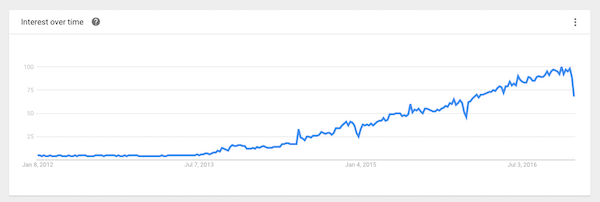
\includegraphics[height=1.1in]{docker}
\caption{Gráfico de utilzação do docker entre os anos 2012 e 2016.}
\label{fig:utilizacao-docker}
\end{figure}

A velocidade de desenvolvimento e implantação de um micro-serviço, permite e incentiva a implementação e estudo dos mesmos. Segundo Adrian micro-serviços possuem características em comum, como: implantação com pouca frequência, novas versões implantadas automaticamentes, orquestração de uso geral não é necessário, uma vez que, sistemas inteiros são implantados com todas as partes ao mesmo tempo, arquiteturas utilizam centenas de micro-serviços, e cada publicação, é altamente customizada (STENBERG, 2015).

Implantar a Aquitetura de Micro-serviços em empresas, irá proporcionar diferentes benefícios para a estrutura de negócio como: usufruir de liberdade maior para o desenvolvimento de serviços de modo independente, implantar aplicações automaticamente através de ferramentas de integração contínua, como Hudson, Jenkins e outras, possibilitar utilização de códigos escritos em linguagens diferentes para diferentes serviços, utilizando comunicação REST através de JSON ou XML, facilitar a ampliação e integração de micro-serviços com serviços terceirizado, atráves de APIs, organizar o código em função de capacidades de negócio, dando mais visão das ofertas e necessidades dos clientes. Dentre todos os benefícios citados, também é possível fazer o gerenciamento de falhas, o que significa que, se um serviço venha a falhar, os outros continuarão funcionando. Através dos micro-serviços, é possível identificar falhas com mais eficiência, visto que, o particionamento favorece uma visão mais detalhada de cada serviço (PELOI, 2016).

Assim como existem os pontos positivos, existem também os negativos, tudo tem seu uso ideal. Em uma publicação feita por Silveira (2016), ele diz que micro-serviços não são uma bala de prata que resolverá todos os problemas de um projeto. A arquitetura de micro-serviços visa o particionamento da aplicação com coesão, entretanto, dependendo da quantidade de partições existentes, torna-se dificultoso a implantação dos mesmos, pelo fato de serem muitos. Além da quantidade de micro-serviços para se implantar, também o cuidado pelas mesmas será maior, pois ao invés de dar manutenção em uma aplicação, aqui serão várias.

Este trabalho têm por objetivo, preencher a lacuna a respeito do desenvolvimento de um micro-serviço, fazendo com que, utilizando-se de ferramentas existentes, seja fácil a criação de uma estrutura para micro-serviços. No Artigo IoT - Internet das coisas de Marques (2017), é desenvolvido uma estrutura de IoT, onde tem-se por objetivo, a comunicação dos dispositivos com aplicações Web, que ficarão encarregadas de compartilhar informações dos mesmos. Durante este trabalho serão criados micro-serviços que posteriormente abrirá possibilidades para integração de dispositivos IoT com micro-serviços, fechando assim, uma estrutura fexível para automações residenciais, entretanto, é título para um próximo trabalho.


% You must have at least 2 lines in the paragraph with the drop letter
% (should never be an issue)
I wish you the best of success.

\hfill mds
 
\hfill 13 de Maio de 2017

\subsection{Revisão bibliográfica}

Segundo dados de Richardson(2014), diversas empresas estão utilizando micro-serviços, dentre as citadas estão: Comcast Cable, Uber, Netflix, Amazon, Ebay, SoundCloud, Karma, Groupon, Hailo, Gilt, Zalando, Lending Club, AutoScout24.
Os problemas associados ao desenvolvimento de software em larga escala ocorreram em torno da década de 1960. Na década de 1970 viu-se um enorme aumento de interesse da comunidade de pesquisa para o design de software em suas aplicações e  no processo de desenvolvimento. Nesta década o design foi muitas vezes considerado como uma atividade não associada com a implementação em si, e portanto requerendo um conjunto especial de notações e ferramentas. Por volta da década de 1980, a integração do design nos processos de desenvolvimento contribuiu para uma fusão parcial dessas duas atividades, tornando assim mais difícil fazer distinções puras.

As referências ao conceito de arquitetura de software também começaram a aparecer década de 1980. No entanto, uma base sólida sobre o tema foi estabelecida apenas em 1992 por Perry Wolf (autor do livro “Foundations for the study of software architecture"). Sua definição de arquitetura de software era distinta do design de software, e desde então tem-se gerado uma grande comunidade de pesquisadores estudando as aplicações práticas da arquitetura de software com base em micro-serviços, permitindo  assim que os conceitos sejam amplamente adotados pela indústria e pela academia.

O advento e a difusão da orientação por objetos, a partir dos anos 80 e, em particular, a década de 1990, trouxe sua própria contribuição para o campo da Arquitetura de Software. O clássico por Gamma et ai. abrange a concepção de software orientado a objetos e como traduzi-lo em código que apresenta uma coleção de soluções recorrentes, chamados padrões. Esta ideia não é nova nem exclusiva à Engenharia de Software, mas o livro é o primeiro compêndio a popularizar a idéia em grande escala. Na era pré-Gamma os padrões para soluções OO já estavam sendo utilizado: um exemplo típico de um padrão de projeto arquitetônico em programação orientada a objetos é o Model-View-Controller (MVC), que tem sido um dos insights seminais no desenvolvimento precoce de interfaces gráficas de usuário.(DRAGONI et al., 2016)

Cerca de sete anos atrás a empresa Netflix (provedora global de filmes e séries de televisão via streaming - distribuição de dados, geralmente de multimídia em uma rede através de pacotes) começou a migrar suas aplicações legadas para uma arquitetura baseada em APIs (Interface de programação de aplicativos) hospedadas na nuvem (local para armazenamento de dados online) da Amazon (empresa transnacional de comércio electrónico dos Estados Unidos com sede em Seattle), influenciando assim, o crescimento de uma ideologia na área de desenvolvimento de softwares que foi batizada pelo nome de “micro-serviço”.

Uma investigação realizada pela empresa Cisco (Companhia sediada em San José, Califórnia, Estados Unidos da América) em 2016 revela que, apesar de toda a euforia sobre a Internet das Coisas, o consumo de de vídeo via internet gera 63\% do tráfego global. A expectativa é que essa marca chegue a 79\% até 2020 e o tráfego de dados gerado por vídeos em resolução Ultra HD subirá de 1.6\% para 20.7\% do total em 2020. Um levantamento realizado pela Cisco VNI Mobile 2016 mostra que os dispositivos IoT mais simples geram uma quantidade de dados equivalentes a 7 veze o que é produzido por um celular comum (não um smartphone). Demandando pouco das redes de telecomunicações, os dispositivos IoT não representarão um grande pessoa para os provedores de infraestrutura na América Latina (IDC, 2016). 

Segundo o relatório “The State of Internet” de 2016, da Akamai (Empresa de Internet americana, sediada em Cambridge, Massachusetts), o país melhor colocado na faixa de redes com banda igual ou maior a 15 Mb/s é o Chile - 4,4\% de seus serviços de Internet atingem essa marca. Entretanto, para chegar a essa posição, o Chile investiu pesadamente entre 2014 e 2015, conseguindo crescer 150\% de um ano para outro. O Uruguai fica logo abaixo, com 4,1\% de sua Internet na faixa dos 15 Mb/s. Atualmente no Brasil, somente 1,1\% dos serviços atingem esta marca.

Na arquitetura de microserviços, se quisermos que um aplicativo seja colocado em esteróides, ele pode ser feito sem afetar outros serviços. Podemos apenas começar a executar este serviço específico em um hardware mais forte. Um microservice único pode ser atualizado nesta arquitetura, sem afetar outros ... a única condição é que o sistema de tempo de execução suporta isso. Cada microservice em uma plataforma pode ser desenvolvido em uma linguagem diferente - Java, C, C ++, Python, etc Governança granular é possível para cada microservice porque não tem dependência em outro. Ele pode ser monitorado e governado separadamente. Essa arquitetura descentraliza o gerenciamento de dados, uma vez que cada microserviço pode armazenar seus dados de uma maneira que se adapte a ele. Arquitetura Microservice suporta automação. É possível mover montagens inteiras de microservices de um ambiente de implementação para outro apenas usando as configurações de perfil com um único clique. Eles são muito mais resistentes do que as aplicações tradicionais. Isto é devido ao fato de que uma única aplicação pode ser retirada de um monte de aplicativos microservices, como estes são independentes uns dos outros.

A arquitetura do microservice tem suas vantagens óbvias e aquela é a razão porque assim que muitos negócios e serviços públicos proeminentes como Netflix, eBay, Amazon, o serviço digital do governo BRIT NICO, realestate.com.au, para diante, Twitter, Paypal, Gilt, Bluemix, Soundcloud , The Guardian, etc, apenas para citar alguns, todos se graduaram de arquitetura monolítica a microservices. Embora este seja o caso, assim como não há um plano perfeito, não há nenhuma arquitetura perfeita. O que funciona sob uma circunstância particular pode se tornar o gargalo em outro.

\subsubsection{Tecnologias para gerenciamento de Micro-serviços}
Neste trabalho será utilizado no Back-end a tecnologia do netflix Service Discovery (Eureka), e para comunicar com este serviço será utilizado o circuito integrado Nodemcu Esp8266. Existem outras bibliotecas que podem trabalhar em conjunto com o Eureka, algumas são: Circuit Breaker (Hystrix), Intelligent Routing (Zuul) and Client Side Load Balancing (Ribbon). 

\subsubsection{Zuul}
Zuul é a ''porta da frente'' para todas as requisições de dispositivos e sites para o back-end. O mesmo foi construído para permitir roteamento dinâmico, monitoramento, resiliência e segurança. O Zuul foi desenvolvido pela Netflix pelo fato de que, o volume e a diversidade do tráfego da API do mesmo, resultam em problemas de produção, surgem rapidamente e sem aviso prévio, e a empresa necessitava de um sistema que permita os mesmos mudarem rapidamente o comportamento e reagir a estas situações.
O Zull utiliza uma variedade de diferentes tipos de filtros, que permitem aplicar rapidamente funcionalidades aos serviços de ponta. Esses filtros ajudam a executar as seguintes funções: Autenticação e segurança, identificação de requisitos de autenticação para cada recurso, negação de solicitações indesejadas, insights e monitoramento, rastreamento de dados significativos e estatísticas, a fim de dar uma visão precisa da produção, roteamento dinâmico, encaminhamento dinâmico solicitações para diferentes clusters de backend conforme necessário, stress Testing, aumento gradual de tráfego para um cluster, a fim de avaliar o desempenho, load Shedding, alocação de capacidade para cada tipo de solicitação e liberação de pedidos que excedem o limite, manipulação de resposta estática e construção de respostas diretamente na ponta ao invés de encaminhá-las para um cluster interno.
Dentre os vários componentes que integram a biblioteca do Zuul, estão: Zuul-core que contém funcionalidades a fim de compilar e executar filtros, Zuul-simple que demonstra como construir um aplicativo com zuul-core e Zuul-netflix que adiciona componentes Netflix utilizando Ribbon para solicitações de roteamento. (Zuul, 2014)

\subsubsection{Ribbon}
Ribbon oferece suporte à comunicação entre processos na nuvem, e inclui balanceadores de carga desenvolvidos pela netflix. A tecnologia citada fornece os seguintes recursos: regras de balanceamento de carga múltiplas e conectáveis, integração com a descoberta de serviços, resiliência de falhas incorporada, clientes integrados com balanceadores de carga e configuração de clientes utilizando Archaius. O Ribbon é composto pelos seguintes projetos: Ribbon-core que inclui definições de interface e balanceamento de carga e cliente, implementações de balanceador de carga comuns, integração de cliente com balanceadores de carga e fábrica de clientes. Ribbon-eureka que inclui implementações do balanceador de carga com base no Eureka-client (biblioteca para registro e descoberta de serviços). Ribbon-httpclient que inclui a implementação de balanceamento de carga baseada em JSR-311. (Ribbon, 2014)

\subsubsection{Hystrix}
Em um ambiente distribuído, inevitavelmente algumas das muitas dependências de serviços falharão, e esta biblioteca ajuda a controlar as interações entre serviços distribuídos, adicionando tolerância de latência e lógica de tolerância a falhas. O mesmo faz isso isolando pontos de acesso entre os serviços, interrompendo falhas em cascata através deles, todas as quais melhoram a resiliência geral do sistema. Atualmente, dezenas de bilhões de threads isoladas e centenas de bilhões não isoladas, são executadas utilizando o Hystrix todos os dias na Netflix. Isso resulta em uma melhoria dramática no tempo, atividade e resiliência das aplicações. Hystrix é um projeto desenvolvido também para proteger e controlar a latência e falhas, de dependências acessadas por meio de bibliotecas de terceiros, monitoramento em tempo real, alertas e controle operacional. Quando se trata de micro-serviços, os mesmos contém dezenas de dependências com outros serviços, o que ocasiona que se um deles falhar, e o mesmo não estiver isolado destas falhas externas, corre o risco de também ser afetado. Como exemplo, um aplicativo que dependa de 40 serviços, em que cada serviço tem 99,99\% de disponibilidade, pode se esperar: 99,99 \^ 40 = 99,6\% de tempo de atividade, 0.4\% de 1 bilhão de falhas resulta em 4 milhões de falhas. Mesmo que pequena a possibilidade de falha, se somar a quantidade de micro-serviços ao tempo de indisponibilidade que pode surgir por pequenas falhas, o problema pode ser facilmente escalável fazendo com que assim serviços importantes fiquem até mesmos horas indisponíveis. Quando toda a aplicação está funcionando e configurada de maneira correta, o fluxo de solicitações ocorrer conforme a figura \ref{fig:hystrix-overtime}.

\begin{figure}[h]
\centering
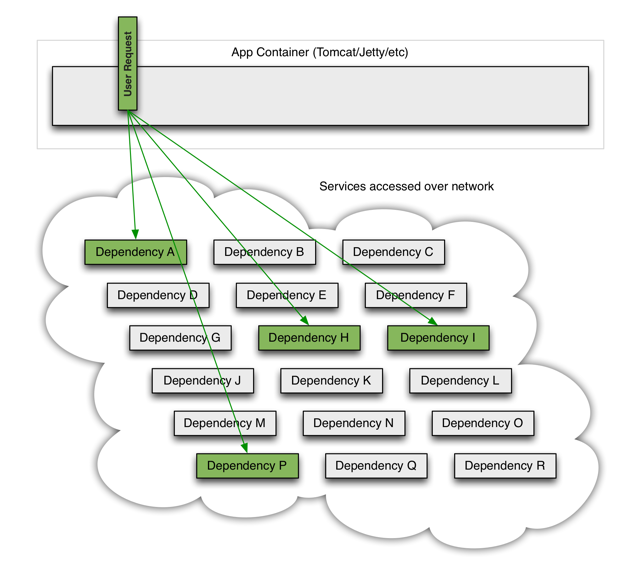
\includegraphics[height=6.2cm]{figura3}
\caption{Wiki Hystrix (Internet Overtime) - 2015).}
\label{fig:hystrix-overtime}
\end{figure}

Quando um dos muitos serviços se torna latente, ele pode bloquear toda a solicitação do usuário, conforme apresentado na figura \ref{fig:hystrix-dimensions-scaling}.

\begin{figure}[h]
\centering
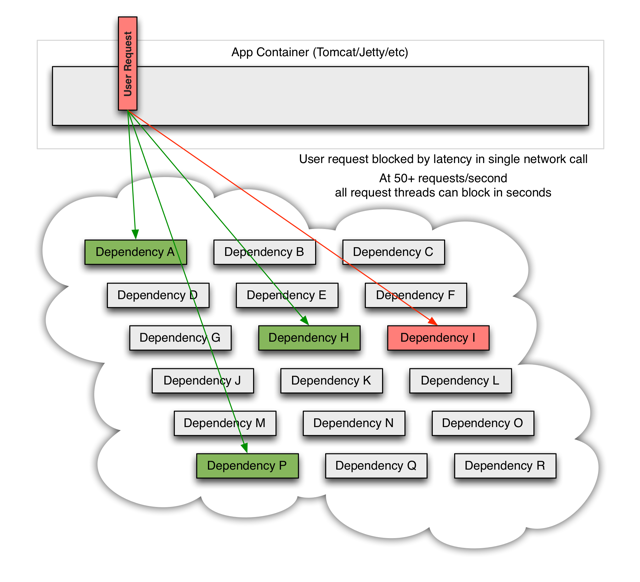
\includegraphics[height=6.2cm]{figura4}
\caption{Wiki Hystrix (3 dimensions to scaling) - 2015).}
\label{fig:hystrix-dimensions-scaling}
\end{figure}

Com tráfego de alto volume, uma única dependência com latência excessiva, pode fazer com que todos os recursos fiquem saturados em segundos. Cada ponto em um aplicativo que atinge a rede, ou em uma biblioteca cliente que pode resultar em solicitações de rede, é uma fonte de falha potencial. Esses aplicativos também podem resultar em latências entre os serviços, causando ainda mais falhas em cascata em todo a aplicação, conforme a figura \ref{fig:hystrix-container}.

\begin{figure}[h]
\centering
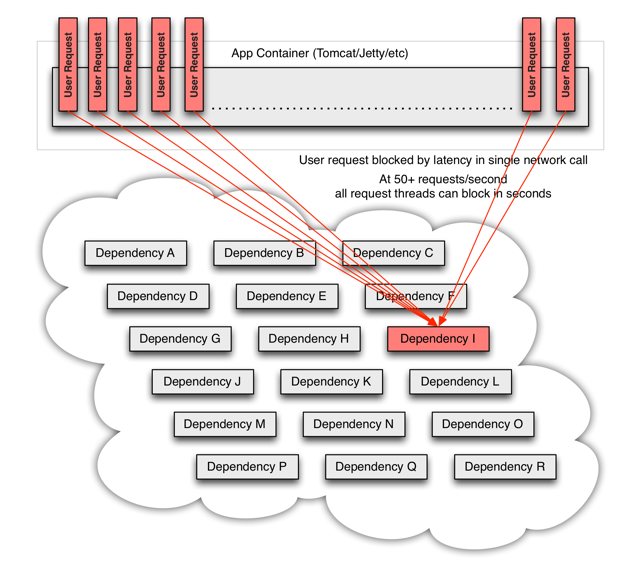
\includegraphics[height=6.2cm]{figura5}
\caption{Wiki Hystrix (Container) - 2015).}
\label{fig:hystrix-container}
\end{figure}

A biblioteca Hystrix subjaz os seguintes princípios de design: impedir que qualquer dependência única utilize todas as threads de usuários de um container (como Tomcat) desperdiçando carga do sistema, fornecer soluções sempre que possível para proteger os usuários contra falhas, utilizar técnicas de isolamento para limitar o impacto de qualquer dependência, otimizar o tempo de descoberta através de métricas, monitoramento e alertas em tempo real, otimizar o tempo de recuperação por meio de propagação de baixa latência de alterações de configuração e, oferecer suporte para alterações de propriedade dinâmicas na maioria dos aspectos do Hystrix, o que permite fazer modificações operacionais em tempo de execução com loops de realimentação de baixa latência, protegendo contra falhas em toda a execução do cliente, não apenas no tráfego da rede. (Hystrix, 2015)

\subsubsection{Eureka + Spring Cloud}
Spring Cloud fornece integrações Netflix OSS para Spring Boot por meio de auto-configuração, e vinculação ao Spring Environment e outros padrões de programação Spring. Dentre os produtos Spring Cloud encontra-se, os clientes Eureka ou Service Discovery, que é um dos princípios fundamentais de uma arquitetura baseada em micro-serviços. Configurar um micro-serviço é trabalhoso, pois envolve diversas técnicas de descoberta e registro de serviços, e com o Service Discovery da Netflix, torna-se eficiente este trabalho pois com poucas anotações Java consegue-se criar uma aplicação simples Eureka. 

Eureka também vem com um componente de cliente baseado em Java, o cliente Eureka, que torna as interações com o serviço muito mais fácil. O cliente também tem um balanceador de carga incorporado, que faz balanceamento de carga round-robin (Algoritmos simples de agendamento e escalonamento de processos) básico. Quando um cliente se registra no Eureka, o mesmo fornece metadados como host e porta, dentre outras informações que podem ser encontradas na documentação. Se o registro falhar durante a configuração, a instância da aplicação é removida do registro. Em resumo, o Eureka é um serviço baseado em REST (Representational State Transfer), que é utilizado principalmente na AWS (Amazon Web Services), para localizar serviços com a finalidade de balanceamento de carga, e failover (tolerância a falhas) de servidores de camada intermediária. 

A Amazon possui um produto chamado AWS ELB (Amazon Web Services Elastic Load Balancer), que é uma solução de balanceamento de carga para serviços de ponta, expostos ao tráfego web do usuário final, e a diferença entre o mesmo e o produto da Netflix, é que o Eureka preenche a necessidade de balanceamento de carga médio. Embora teoricamente pode-se colocar serviços de nível intermediário junto com o AWS ELB, no EC2 classic (Elastic Compute Cloud), pode-se expor à rede externa, e perder toda a utilidade dos grupos de segurança AWS. O AWS ELB  também possui uma solução de balanceamento de carga em proxy (servidor intermediário para requisições entre cliente e servidor final) tradicional, enquanto no Eureka, o balanceamento ocorre no nível da instância, servidor e host. As instâncias do cliente sabem todas as informações sobre quais aplicações precisam conversar.

Na Netflix, além de desempenhar um papel crítico no balanceamento de carga de nível médio, o Eureka é utilizado para os seguintes fins: implementações com Netflix Asgard, um serviço para fazer atualizações de serviços de forma rápida e segura, registro e exclusão de instâncias e transporte de metadados específicos de aplicativos adicionais sobre serviços. Dentre os motivos para utilizar o Eureka está o fato de que, o mesmo provê uma solução para balanceamento de carga round-robin simples, e quando não pode-se expor o tráfego das aplicações externamente com o AWS ELB, o Eureka resolve este problema.

Com o Eureka, a comunicação é transparente, pois o mesmo fornece informações sobre os serviços desejados para comunicação, mas não impõe quaisquer restrições sobre o protocolo ou método de comunicação. Exemplificando, pode-se utilizar o Eureka para obter o endereço do servidor destino e utilizar protocolos como thrift, http(s) ou qualquer outro mecanismos RPC (Remote Procedure Call) que permite fazer conexões ou chamadas por espaço de endereçamento de rede. 

\subsubsection{Modelo Arquitetural Eureka}
O modelo arquitetural implantado na Netflix utilizando o Eureka é descrita na figura \ref{fig:wiki-eureka-est}. Existe um cluster por região que conhece somente instâncias de sua região. Há pelo menos um servidor Eureka por zona para lidar com falhas da mesma. Os serviços se registram e, em seguida, a cada 30 segundos enviam os chamados ''batimentos cardíacos'' ou requisições para renovar seus registros. Se o cliente não renovar o registro, ele é retirado do servidor em cerca de 90 segundos. As informações de registro e renovações são replicadas para todos as conexões no cluster. Os clientes de qualquer zona podem procurar as informações do registro para localizar seus serviços que podem estar em qualquer zona e fazer chamadas remotas.

Para serviços não baseados em Java, têm-se a opção de implementar a parte do cliente, utilizando o protocolo REST desenvolvido para o Eureka ou executar um ''side car'' que é uma aplicação Java com um cliente embutido Eureka, que manipula os registros e conexões. Quando se trabalha com serviços em nuvem, pensar em resiliência se torna ímprobo. Eureka se beneficia dessa experiência adquirida, e é construído para lidar com falha de um ou mais servidores do mesmo.

\begin{figure}[h]
\centering
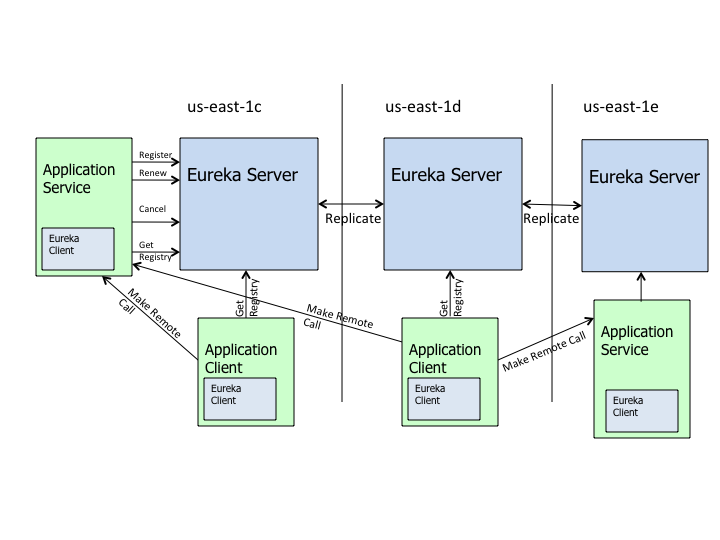
\includegraphics[height=6.2cm]{figura6}
\caption{Wiki Eureka - 2015).}
\label{fig:wiki-eureka-est}
\end{figure}
 



% needed in second column of first page if using \IEEEpubid
%\IEEEpubidadjcol

\subsection{Desenvolvimento}

\subsection{Iniciando com Eureka Client}

Este trabalho tem por objetivo o a pesquisa e desenvolvimento de uma estrutura de micro-serviços. Como o projeto será baseado em Java, inicialmente será criado um projeto que utilizará maven, para gerenciamento de dependências, e o Eureka Client para descoberta de serviços. Após a criação de um projeto utilizando Maven, será incluso o groupId org.springframework.cloud e o artifactId spring-cloud-starter-eureka no arquivos de configuração das dependências.

Quando um cliente se registra com o Eureka, ele fornece meta-dados sobre si, indicador de estado ou saúde, página inicial, dentre outros. Eureka recebe mensagens heartbeat (disponibilidade) de cada instância pertencente a um serviço, e se algum heartbeat falhar, a instância é removido do registro.
Para inicializar um projeto com Eureka Client, será utilizado algumas anotações Java fornecidas pelo Eureka descritas a seguir: @Configuration, para utilizar recursos do projeto Spring Config, para facilitar configurações de projetos Spring baseado em Java, @ComponentScan para buscar componentes em pacotes java, @EnableAutoConfiguration para ativar as configurações automáticas internas, @EnableEurekaClient para ativar a descoberta de serviços do Eureka, @RestController para criar um controlador Rest (Representational State Transfer), @RequestMapping para mapear as rotas da aplicação.

\begin{verbatim}
@Configuration
@ComponentScan
@EnableAutoConfiguration
@EnableEurekaClient
@RestController
public class Application {

    @RequestMapping("/")
    public String home() {
        return "Hello world";
    }

    public static void main(String[] args) {
        new SpringApplicationBuilder
          (Application.class).web(true)
          .run(args);
    }
}
\end{verbatim}

Para que possa surtir efeito na aplicação, é necessário fazer ajustes nas configurações do Eureka, dentro do diretório resources da aplicação Java. Esta configuração é feita dentro de um arquivo Application.yml.

\begin{verbatim}
  Eureka
   cliente:
     ServiceUrl:
       DefaultZone: 
        http://localhost:8761/eureka/ 
\end{verbatim}

Neste arquivo de configuração, encontra-se uma peculiaridade. O DefaultZone é a URL do serviço Eureka para qualquer cliente. O nome do aplicativo padrão (ID de serviço), o host e a porta podem ser acessadas respectivamente pelas variáveis de ambientes: \${spring.application.name} , \${spring.application.name} e \${server.port}.
A anotação Java @EnableEurekaClient faz com que, a aplicação corrente se registre no Eureka, para que assim possa localizar outros serviços.

\subsection{Status e Saúde do serviço}

Com a página de status e os indicadores de integridade de uma instância do Eureka, é possível visualizar informações do serviço. Para acessar os indicadores de saúde, deve-se configurar as rotas padrões de acesso a mesma. Por padrão, o eureka utiliza a conexão do cliente, para determinar se está ativo. Caso não seja utilizado o Discovery Client, não será propagado o status de verificação de integridade atual do serviço. Para que os indicadores de saúde e status da aplicação funcionem corretamente, devem ser feitas as seguintes configurações:

\begin{verbatim}
eureka:
  instance:
    statusPageUrlPath: 
      ${management.context-path}/info
    healthCheckUrlPath: 
      ${management.context-path}/health
  client:
    healthcheck:
      enabled: true
\end{verbatim}

Para conseguir utilizar mais recursos e obter mais informações sobre o status da aplicação, a aplicação deve implementar seu próprio controle de integridade que se encontra no pacote com.netflix.appinfo.HealthCheckHandler

\subsection{Alterando o ID da instância Eureka}

Uma instância registrada no Eureka possui seu ID, que identifica o serviço que está no mesmo. O Spring Cloud Eureka fornece o seguinte padrão de configuração: \$\{spring.cloud.client.hostname\}:\$\{spring.application.name\}:
\$\{spring.application.instance\_id:\$\{server.port\}\}. Como exemplo a URL fica da seguinte maneira: myhost:myapp:8080

\subsection{Iniciando com EurekaClient}

O próximo passo para utilizar o Eureka Server para coreografar os micro-serviços, é utlizar o Eureka Client, que pode ser utilizado para descobrir instâncias do mesmo. Para fazer isto utilizando o framework, primeiramente é necessário incluir a dependência do EurekaClient, e criar um método que busque as instâncias registradas no Eureka.

\begin{verbatim}
@Autowired
private EurekaClient discoveryClient;

public String serviceUrl() {
  InstanceInfo instance = 
    discoveryClient
    .getNextServerFromEureka
      ("STORES", false);
    return instance.getHomePageUrl();
}
\end{verbatim}

Não necessariamente é preciso utilizar o EurekaClient. Também pode-se utilizar o DiscoveryClient. A diferença entre os dois, está na maneira de como é utilizado.

\begin{verbatim}
@Autowired
private DiscoveryClient discoveryClient;

public String serviceUrl() {
    List<ServiceInstance> list = 
      discoveryClient.getInstances
        ("STORES");
    if (list != null && list.size() > 0 ) {
        return list.get(0).getUri();
    }
    return null;
}
\end{verbatim}

\subsection{Performanece de registro no Eureka}

Registrar um serviço no Eureka pode ser considerado um pouco lento, pelo fato de que, ser uma instância também envolve um heartbeat periódico para o registro, com duração padrão de 30 segundos. Um serviço não estará disponível para descoberta por clientes, enquanto uma intância tenha todos os metadados em seu cache local. Para alterar o período em que isto ocorre, pode ser configurado através da propriedade eureka.instance.leaseRenewalIntervalInSeconds. Entretanto, em produção, não deve ser alterado este padrão pelo fato de que, existem alguns cálculos internos do Eureka, que fazem suposições de renovação de locação.

\subsection{Zonas Eureka}

Primeiramente, para se configurar uma zona Eureka, é necessário ter certeza de que existem servidores Eureka implantados em cada zona e que eles são pares uns dos outros. Em seguida, precisa-se informar em qual zona o mesmo está. Para fazer isto será utilizado a propriedade metadataMap. E isto pode ser feito da seguinte forma:

\begin{verbatim}
eureka.instance.metadataMap.zone = zone1
eureka.client.preferSameZoneEureka = true
\end{verbatim}

\subsection{Primeiros passos com Eureka Server}

Como este projeto é baseado em Java no backend, e utiliza maven como gerenciador de dependências, será incluso nas configurações de dependências Maven o groupId org.springframework.cloud e o artifactId spring-cloud-starter-eureka-server. Com esta dependência adicionada, será possível utilzar o Eureka Server.

Após adicionar esta dependência, será criado a classe principal, que se encarregará de iniciar a aplicação Eureka Server. Utilizando-se da anotação @EnableEurekaServer fornecida pelo framework, e seguindo o padrão utilizado no Eureka Client para iniciar a aplicação, é possível ver um resultado. Um exemplo de código pode ser visto a seguir.

\begin{verbatim}
@SpringBootApplication
@EnableEurekaServer
public class Application {
  public static void main(String[] args) {
      new SpringApplicationBuilder
        (Application.class).web(true)
        .run(args);
  }
}
\end{verbatim}

\subsection{Modo Autônomo}

A combinação entre o cliente e servidor Eureka, e as pulsações para verificação de disponibilidade entre os mesmos, tornam o servidor Eureka
resiliente à falhas, contanto que haja algum tipo de monitoramento para mantê-lo funcionando. No modo autônomo, pode-se prefirir desativar o comportamento padrão do lado do cliente, para que ele não continue tentado alcançar seus pares caso haja falha. Para isto será feito diversas configurações como pode ser visto a seguir.


\begin{verbatim}
server:
  port: 8761

eureka:
  instance:
    hostname: localhost
  client:
    registerWithEureka: false
    fetchRegistry: false
    serviceUrl:
      defaultZone: 
        http://${eureka.instance.hostname}
        :${server.port}/eureka/
\end{verbatim}

Acima foi apresentado as seguintes configurações: port que configura a porta em que será instalado a aplicação, hostname para identificar o nome do host, registerWithEureka que indica se a própria aplicação do Eureka se registrará em si mesma, e fetchRegistry que diz se o Eureka buscará registros associados a eles que ainda estão executando, porém ainda não registradas no Eureka.
Com o Eureka, os registros podem ser ainda mais resistentes e disponíveis, executando várias instâncias e pedindo-lhes para se registrarem uns com os outros. Tudo o que precisa para fazê-lo é configurar o serviceUrl dos pares.

\begin{verbatim}
---
spring:
  profiles: peer1
eureka:
  instance:
    hostname: peer1
  client:
    serviceUrl:
      defaultZone: http://peer2/eureka/

---
spring:
  profiles: peer2
eureka:
  instance:
    hostname: peer2
  client:
    serviceUrl:
      defaultZone: http://peer1/eureka/
\end{verbatim}

Neste exemplo, o serviço pode ser utilizado para executar o mesmo servidor em 2 hosts (peer1 e peer2), executando-o em diferentes perfis Spring. É possível utilizar esta configuração para testar a descoberta dos pares em um único host, manipulando neste caso em servidor Linux, o arquivo hosts para resolver os nomes de host que pode ser encontrado dentro do diretório /etc/hosts.

Em alguns casos, é preferível que o Eureka utilize os endereços IP dos serviços, ao invés do nome do host. Para isto deve ser definido a configuração eureka.instance.preferIpAddress como true, e quando a aplicação se registrar com o Eureka, o mesmo utilizará seu endereço IP ao invés do nome de host.

\subsection{Clientes Hystrix}

Segundo Fowler (2016), é comum que os sistemas de software façam chamadas remotas para software em execução em diferentes processos, provavelmente em máquinas diferentes em uma rede. Uma das grandes diferenças entre chamadas em memória e chamadas remotas é que, chamadas remotas podem falhar ou travar sem uma resposta, até que algum limite de tempo limite seja atingido. Devido a diversos problemas que podem ocorrer na arquitetura de micro-serviços, a Netflix criou a biblioteca chamada Hystrix, que impelementa o padrão disjuntor que interromple automáticamente o serviço quando ocorre falhas. Uma falha de serviço no nível inferior de serviços pode causar falha em cascata em todo o caminho até o usuário. No Hystrix o padrão de limite de falhas são 20 em 5 segundos, e quando ocorre o circuito é aberto e a chamada não é feita, isto pode ser visto na figura \ref{fig:figura7}

\begin{figure}[h]
\centering
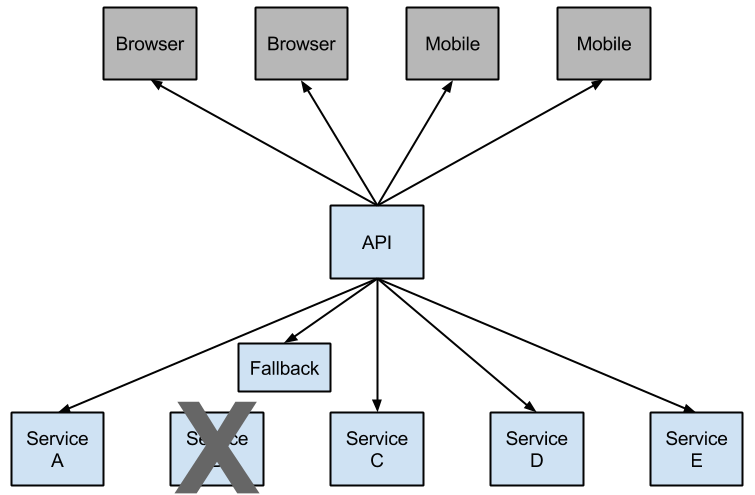
\includegraphics[height=4.2cm]{figura7}
\caption{Fallback Hystrix em falhas em cascata.}
\label{fig:figura7}
\end{figure}

\subsection{Primeiros passos com Hystrix}

Para utilizar o Hystrix, precisa ser incluso a dependência com o groupId org.springframework.cloud e o artifactId spring-cloud-starter-Hystrix, e a anotação @EnableCircuitBreaker na classe principal.

\begin{verbatim}
@SpringBootApplication
@EnableCircuitBreaker
public class Application {

    public static void main(String[] args) {
        new SpringApplicationBuilder
          (Application.class).web(true)
          .run(args);
    }

}

@Component
public class StoreIntegration {

    @HystrixCommand
      (fallbackMethod = "defaultStores")
    public Object getStores
      (Map<String, Object> parameters) {
        //do stuff that might fail
    }

    public Object defaultStores
      (Map<String, Object> parameters) {
        return /* something useful */;
    }
}
\end{verbatim}

No exemplo de código acima, foi implementando uma classe que se contém um método que buscará os serviços, e para isto foi utilizado a anotação @HystrixCommand. É possível ativar as métricas Hystrix e a central de gerenciamento do mesmo adicionando as dependências abaixo. O endpoint para acesso ao gerenciador é /hystrix.stream.

\begin{verbatim}
<dependency>
    <groupId>
      org.springframework.boot
    </groupId>
    <artifactId>
      spring-boot-starter-actuator
    </artifactId>
</dependency>
<dependency>
    <groupId>
      org.springframework.cloud
    </groupId>
    <artifactId>
    spring-cloud-starter-hystrix-dashboard
    </artifactId>
</dependency>
\end{verbatim}

\subsection{Ribbon}

Ribbon é um  balanceador de carga do lado do cliente, que fornece controles sobre o comportamento dos clientes HTTP e TCP. Uma observação importante é que a anotação @FeignClient já utiliza Ribbon, fazendo com que assim seja desnecessário a utilização do Ribbon, entretanto, quando for preciso um controle mais versátil sobre a tecnologia é optável a utilização do mesmo.

Para incluir o ribbon no projeto, será utilizado o mesmo padrão de configurações feito anteriormente. O que será alterado é o artifactId da dependência maven, que agora será utilizado spring-cloud-starter-ribbon, e para configurar o cliente Ribbon criado uma classe de configuraçao e será anotado com @RibbonClient. 

\begin{verbatim}
@Configuration
@RibbonClient(name = "foo", 
  configuration = FooConfiguration.class)
public class TestConfiguration {
}
\end{verbatim}

\subsection{FeignClient}

FeignClient é uma biblioteca que faz com que clientes de serviços web sejam escritos de forma mais fácil. Para utilizá-lo é preciso instalar a dependência spring-cloud-starter-feign, e anotar a classe principal com @EnableFeignClients. O mesmo provê suporte para anotações Spring MVC, e por utilizar o mesmo conversor de mensagens HTTP que o Spring Web, é integrada com Hystrix para fornecer um cliente com balanceamento de carga.

\begin{verbatim}
@Configuration
@ComponentScan
@EnableAutoConfiguration
@EnableEurekaClient
@EnableFeignClients
public class Application {
  public static void main(String[] args) {
      SpringApplication
        .run(Application.class, args);
  }
}
\end{verbatim}

Ao anotar uma interface com @FeignClient, pode ser mapeado os métodos para que consiga acesso a endpoints da biblioteca. O nome do método será qualificado e aplicado ao contexto da aplicação, fazendo com que assim não seja implementado corpo ao método pois será apenas repassados chamadas REST.

\begin{verbatim}
@FeignClient("stores")
public interface StoreClient {
  @RequestMapping(method = 
    RequestMethod.GET, 
    value = "/stores")
    List<Store> getStores();

    @RequestMapping(method = 
      RequestMethod.POST, 
      value = "/stores/{storeId}", 
      consumes = "application/json")
    Store update(
     @PathVariable("storeId") Long storeId, 
     Store store);
}
\end{verbatim}

Cada Cliente Feign faz parte de um conjunto de componentes que trabalham juntos, para comunicar-se via HTTP. O Spring Cloud permite com que se tenha controle total sobre clientes Feign, declarando uma classe de configuração que implemente determinados métodos do FeignClient. Duas das possíveis configuração, são: modificar o padrão de Contrato que o FeignClient utiliza para que assim seja personalizado o padrão de comunicação REST que o mesmo utiliza e modificar o método de autenticação do FeignClient.

\begin{verbatim}
@Configuration
public class FooConfiguration {
  @Bean
  public Contract feignContract() {
      return new feign.Contract.Default();
  }

  @Bean
  public BasicAuthRequestInterceptor 
    basicAuthRequestInterceptor() {
     return new BasicAuthRequestInterceptor
        ("user", "password");
  }
}
\end{verbatim}

\subsection{Zuul}

Até neste capítulo, foi falado de rotas e endpoints, mas ainda não foi explorado a essencialidade de utilizar rotas. Roteamento é uma parte fundamental de uma arquitetura de micro-serviços, pelo fato de que, uma uri (identificador uniforme de recursos) pode ser mapeado de acordo com sua utilidade. Como exemplo, uma uri \/api\/usuario é mapeado para o serviço de usuário, \/api\/vendas pode ser mapeado para o serviço de vendas de uma loja. Zuul é um roteador com balanceamento de carga básico. A empresa Netflix atualmente utiliza o Zuul para os seguintes desígnios: autenticação, insights teste de stress da api, Canary test que segundo Sato (2014) é uma técnica para reduzir o risco de introduzir uma nova versão de software na produção lentamente lançando a mudança para um pequeno subconjunto de usuário antes de lança-la em toda a infra-estrutura e torná-la disponível para todos, roteamento dinâmico, serviço de migração, divisão de carga, segurança, manipulação de respostas e gestão de tráfego de dados.

Para incluir o Zuul em um projeto utilizando os padrões aplicados até neste capítulo, é necessário utilizar o artifactId spring-cloud-starter-zuul, e para habilitá-lo, a classe principal deve ser anotada com @EnableZuulProxy, e este encaminhará chamadas locais para o serviço adequado. Para que de acordo com a rota seja chamado o serviço desejado deve ser configurado no arquivo de configurações principais application.yml, e para ignorar demais serviços utiliza-se a propriedade zuul.ignored-services. Abaixo está um exemplo da utilizaçao da mesma.

\begin{verbatim}
 zuul:
  ignoredServices: '*'
  routes:
    produtos: /meus-produtos/**
\end{verbatim}

Para obter um controle mais refinado sobre determinadas rotas, pode-se especificar o caminho e o serviceId.

\begin{verbatim}
 zuul:
  routes:
    produtos:
      path: /meus-produtos/**
      serviceId: produtos_service
\end{verbatim}

Isto significa que quando ocorrer uma chamado para a rota \"\/myprodutos\", o mesmo será encaminhado para o serviço \"produtos\_service\". Se for desejável especificar uma URL para uma localização física do serviço, pode ser feito da seguinte maneira.

\begin{verbatim}
 zuul:
  routes:
    produtos:
      path: /produtos/**
      url: 
       http://exemple.com/produtos_service
\end{verbatim}

As configurações de rotas feitas até o momento, não são executadas como um HystrixCommand ou balancedas com Ribbon. Para conseguir isto, deve-se especificar um serviço de rota e criar um cliente Ribbon para o serviceId. Abaixo, um exemplo de configuração para o mesmo.

\begin{verbatim}
zuul:
  routes:
    produtos:
      path: /meus-produtos/**
      serviceId: produtos

ribbon:
  eureka:
    enabled: false

produtos:
  ribbon:
    listOfServers: exemplo.com,faype.com
\end{verbatim}

\subsection{Migração de aplicações}

Um padrão comum ao migrar um serviço Web existente, é remover endpoints antigo, e lentamente substitui-los por novas implementações. O proxy Zuul é uma ferramenta extremamente útil para isto, pelo fato de que, pode-se utilizá-lo para lidar com todo o tráfego de clientes antigos, mas lidar com solicitações para novos. Abaixo segue um exemplo de configuração.

\begin{verbatim}
 zuul:
  routes:
    primeiro:
      path: /primeiro/**
      url: http://primeiro.exemplo.com
    segundo:
      path: /segundo/**
      url: forward:/segundo
    terceiro:
      path: /terceiro/**
      url: forward:/3rd
    legacy:
      path: /**
      url: http://teste.exemplo.com
\end{verbatim}

Ao processar as solicitações de entrada, parâmetros de consulta são  decoficados para que os mesmos possam estar disponíveis para possíveis modificações nos filtro Zuul. Estes são recodificados aos reconstruir o pedido backend nos filtros de rota. O resultado pode ser diferente da entrada original, principalmente se o mesmo foi codificando utilizando por exemplo na linguagem Javascript a função encodeURIComponent(). Isto não causa problemas na maiorias dos casos, entretanto, algumas aplicações web podem exigir codificação de url para consultas complexas. Para forçar a codificação original da url, é possível utilizar a configuração zull.forceOriginalQueryStringEncoding definindo-à como true.


\subsection{RxJava com Spring MVC}

RxJava é uma implementação Java VM de extensões reativas : uma biblioteca para compor programas assíncronos e baseados em eventos utilizando sequências observáveis. (NETFLIX, 2017).

Spring Cloud fornece suporte para observables que em RxJava é um objeto que implementa a interface Observable que em seguida, este assinante reage a qualquer item ou sequência de itens que o objeto Observable emite. Esse padrão facilita operações simultâneas porque não precisa bloquear enquanto espera que o Observable emita objetos, mas ao invés disto, cria uma sentinela na forma de assinante que está pronto para reagir apropriadamente em qualquer tempo futuro que o Observable gere (REACTIVEX, 2016). Utilizando o Spring Cloud pode-se retornar objetos rx.Single, rx.Observale e SSE (Eventos enviados pelo servidor) que é uma tecnologia pelo qual um navegador recebe atualizações de um servidor via HTTP. Abaixo está dois exemplos, segundo a Netflix (2017) de como utilizá-los.

\begin{verbatim}
@RequestMapping(method =
  RequestMethod.GET, value = "/multiple")
  public Single<List<String>> multiple() {
    return Observable
      .just("multiple", "values")
      .toList().toSingle();
}

@RequestMapping(
    method = RequestMethod.GET, 
    value = "/responseWithObservable")
 public ResponseEntity<Single<String>> 
    responseWithObservable() {

 Observable<String> observable = 
 Observable.just("single value");
 HttpHeaders headers = new HttpHeaders();
 headers
  .setContentType(APPLICATION_JSON_UTF8);
 return new ResponseEntity<>(
      observable.toSingle(), 
    headers, HttpStatus.CREATED);
}
\end{verbatim}

\subsection{Motivação de uso das tecnologias apresentadas}

Até o prezado momento, foram apresentados diversas tecnologias, entretanto, fica a questão sobre o por que de tantas tecnologias. e a resposta é clara e objetiva. Para que se tenham micro-serviços, é necessário a utilização de um recurso para a orquestração dos mesmos, neste caso, entra o Eureka. Quando se tem micro-serviços, é necessário a centralização dos mesmos para que não fique espalhados e perdidos em hosts ou portas diferentes, surge a necessidade de um gateway, neste caso, o Zuul. A partir do momento que são integrados muitos micro-serviços, torna-se difícil o gerenciamento da configuração dos mesmos, surgindo a necessidade de um mecanismo para fácil configuração e integração de aplicações, por isto, foi apresentado o Spring Config. Após tudo isto, surge ainda um problema, o balanceamento de carga, um problema abrangente quando se trabalha com aplicações distribuidas. Surge então, a motivação de utilizar o Ribbon para distribuição de carga. Com tudo isto configurado, ainda não se tem garantia precisa de disponibilidade da aplicação, fazendo com que, se caso ocorrer um problema em um micro-serviço, necessite de uma tecnologia que resolva esta questão, fazendo assim necessário a utilização do Hystrix. A motivação de apresentar tecnologias Spring Cloud e Netflix, como citado na introdução deste trabalho, é o fato da experiência e sucesso por parte dos mesmos em aplicações distribuidas.


\subsection{Conclusão}
\subsubsection{sub2}


% An example of a floating figure using the graphicx package.
% Note that \label must occur AFTER (or within) \caption.
% For figures, \caption should occur after the \includegraphics.
% Note that IEEEtran v1.7 and later has special internal code that
% is designed to preserve the operation of \label within \caption
% even when the captionsoff option is in effect. However, because
% of issues like this, it may be the safest practice to put all your
% \label just after \caption rather than within \caption{}.
%
% Reminder: the "draftcls" or "draftclsnofoot", not "draft", class
% option should be used if it is desired that the figures are to be
% displayed while in draft mode.
%
%\begin{figure}[!t]
%\centering
%\includegraphics[width=2.5in]{myfigure}
% where an .eps filename suffix will be assumed under latex, 
% and a .pdf suffix will be assumed for pdflatex; or what has been declared
% via \DeclareGraphicsExtensions.
%\caption{Simulation results for the network.}
%\label{fig_sim}
%\end{figure}

% Note that the IEEE typically puts floats only at the top, even when this
% results in a large percentage of a column being occupied by floats.


% An example of a double column floating figure using two subfigures.
% (The subfig.sty package must be loaded for this to work.)
% The subfigure \label commands are set within each subfloat command,
% and the \label for the overall figure must come after \caption.
% \hfil is used as a separator to get equal spacing.
% Watch out that the combined width of all the subfigures on a 
% line do not exceed the text width or a line break will occur.
%
%\begin{figure*}[!t]
%\centering
%\subfloat[Case I]{\includegraphics[width=2.5in]{box}%
%\label{fig_first_case}}
%\hfil
%\subfloat[Case II]{\includegraphics[width=2.5in]{box}%
%\label{fig_second_case}}
%\caption{Simulation results for the network.}
%\label{fig_sim}
%\end{figure*}
%
% Note that often IEEE papers with subfigures do not employ subfigure
% captions (using the optional argument to \subfloat[]), but instead will
% reference/describe all of them (a), (b), etc., within the main caption.
% Be aware that for subfig.sty to generate the (a), (b), etc., subfigure
% labels, the optional argument to \subfloat must be present. If a
% subcaption is not desired, just leave its contents blank,
% e.g., \subfloat[].


% An example of a floating table. Note that, for IEEE style tables, the
% \caption command should come BEFORE the table and, given that table
% captions serve much like titles, are usually capitalized except for words
% such as a, an, and, as, at, but, by, for, in, nor, of, on, or, the, to
% and up, which are usually not capitalized unless they are the first or
% last word of the caption. Table text will default to \footnotesize as
% the IEEE normally uses this smaller font for tables.
% The \label must come after \caption as always.
%
%\begin{table}[!t]
%% increase table row spacing, adjust to taste
%\renewcommand{\arraystretch}{1.3}
% if using array.sty, it might be a good idea to tweak the value of
% \extrarowheight as needed to properly center the text within the cells
%\caption{An Example of a Table}
%\label{table_example}
%\centering
%% Some packages, such as MDW tools, offer better commands for making tables
%% than the plain LaTeX2e tabular which is used here.
%\begin{tabular}{|c||c|}
%\hline
%One & Two\\
%\hline
%Three & Four\\
%\hline
%\end{tabular}
%\end{table}


% Note that the IEEE does not put floats in the very first column
% - or typically anywhere on the first page for that matter. Also,
% in-text middle ("here") positioning is typically not used, but it
% is allowed and encouraged for Computer Society conferences (but
% not Computer Society journals). Most IEEE journals/conferences use
% top floats exclusively. 
% Note that, LaTeX2e, unlike IEEE journals/conferences, places
% footnotes above bottom floats. This can be corrected via the
% \fnbelowfloat command of the stfloats package.




\section{Conclusion}
The conclusion goes here.





% if have a single appendix:
%\appendix[Proof of the Zonklar Equations]
% or
%\appendix  % for no appendix heading
% do not use \section anymore after \appendix, only \section*
% is possibly needed

% use appendices with more than one appendix
% then use \section to start each appendix
% you must declare a \section before using any
% \subsection or using \label (\appendices by itself
% starts a section numbered zero.)
%


\appendices
\section{Proof of the First Zonklar Equation}
Appendix one text goes here.

% you can choose not to have a title for an appendix
% if you want by leaving the argument blank
\section{}
Appendix two text goes here.


% use section* for acknowledgment
\section*{Acknowledgment}


The authors would like to thank...


% Can use something like this to put references on a page
% by themselves when using endfloat and the captionsoff option.
\ifCLASSOPTIONcaptionsoff
  \newpage
\fi



% trigger a \newpage just before the given reference
% number - used to balance the columns on the last page
% adjust value as needed - may need to be readjusted if
% the document is modified later
%\IEEEtriggeratref{8}
% The "triggered" command can be changed if desired:
%\IEEEtriggercmd{\enlargethispage{-5in}}

% references section

% can use a bibliography generated by BibTeX as a .bbl file
% BibTeX documentation can be easily obtained at:
% http://mirror.ctan.org/biblio/bibtex/contrib/doc/
% The IEEEtran BibTeX style support page is at:
% http://www.michaelshell.org/tex/ieeetran/bibtex/
%\bibliographystyle{IEEEtran}
% argument is your BibTeX string definitions and bibliography database(s)
%\bibliography{IEEEabrv,../bib/paper}
%
% <OR> manually copy in the resultant .bbl file
% set second argument of \begin to the number of references
% (used to reserve space for the reference number labels box)
\begin{thebibliography}{1}

\bibitem{IEEEhowto:kopka}
H.~Kopka and P.~W. Daly, \emph{A Guide to \LaTeX}, 3rd~ed.\hskip 1em plus
  0.5em minus 0.4em\relax Harlow, England: Addison-Wesley, 1999.

\end{thebibliography}

% biography section
% 
% If you have an EPS/PDF photo (graphicx package needed) extra braces are
% needed around the contents of the optional argument to biography to prevent
% the LaTeX parser from getting confused when it sees the complicated
% \includegraphics command within an optional argument. (You could create
% your own custom macro containing the \includegraphics command to make things
% simpler here.)
%\begin{IEEEbiography}[{\includegraphics[width=1in,height=1.25in,clip,keepaspectratio]{mshell}}]{Michael Shell}
% or if you just want to reserve a space for a photo:

\begin{IEEEbiography}{Michael Shell}
Biography text here.
\end{IEEEbiography}

% if you will not have a photo at all:
\begin{IEEEbiographynophoto}{John Doe}
Biography text here.
\end{IEEEbiographynophoto}

% insert where needed to balance the two columns on the last page with
% biographies
%\newpage

\begin{IEEEbiographynophoto}{Jane Doe}
Biography text here.
\end{IEEEbiographynophoto}

% You can push biographies down or up by placing
% a \vfill before or after them. The appropriate
% use of \vfill depends on what kind of text is
% on the last page and whether or not the columns
% are being equalized.

%\vfill

% Can be used to pull up biographies so that the bottom of the last one
% is flush with the other column.
%\enlargethispage{-5in}



% that's all folks
\end{document}


